\documentclass[a4paper,12pt]{article}
\usepackage[a4paper, margin=1in]{geometry} % Sets the paper size to A4 and margins to 1 inch
\usepackage{graphicx}
\usepackage{subcaption} % for subfigures
\usepackage{setspace}		
\usepackage{xcolor,listings} % for typesetting code
\usepackage{enumitem}

% Define SQL listing style
% \lstset{
%     language=SQL,
%     basicstyle=\ttfamily,
%     keywordstyle=\bfseries,
%     commentstyle=\itshape,
%     showstringspaces=false,
%     numbers=left,
%     numberstyle=\tiny,
%     numbersep=5pt,
%     breaklines=true,
%     frame=single,
%     backgroundcolor=\color{gray!10},
%     captionpos=b
% }
\lstset{
    upquote=true,
    language=SQL,
    showspaces=false,
    basicstyle=\ttfamily,
    keywordstyle=\bfseries\color{blue!50},
    numbers=left,
    numberstyle=\tiny,
    commentstyle=\color{gray}
}

\begin{document}


%% Adding logo
\begin{figure}[h]
		\vspace*{-1em}
		\centering
		
\includegraphics[width=0.2\linewidth]{university_logo.png}
		\par
		\vspace*{2em}
		{\Large UNIVERSITY OF CHITTAGONG}
\end{figure}
%% Document information
\begin{center}
		\vspace*{3em}
		\textbf{Department of Computer Science and Engineering} \\
		\bigskip
		Session: 2021-2022 \\
		4th semester \\
		\bigskip
		\begin{tabular}{l l}
		  Assignment No. &: 1\\
		  Course Title &: Database Systems \\
		  Course Code No. &: CSE-413 \\
		\end{tabular}
\end{center}

%% Teacher information
\begin{center}
		\vspace*{3em}
		Submitted to: \\
		\textbf{Dr. Rudra Pratap Deb Nath} \\
		Associate Professor \\
		Department of Computer Science and Engineering \\
		University of Chittagong
\end{center}

%% Student information
\begin{center}
		\vspace*{3em}
		Submitted by: \\
		\textbf{Sanzid Islam Mahi} \\
		ID: 22701065 \\
		Department of Computer Science and Engineering \\
		University of Chittagong
\end{center}




\begin{center}
	\vspace*{3em}
	Date: Jul 02, 2024
\end{center}

\newpage
\section*{Chapter 1}
\subsection*{Part 1}
\subsubsection*{Test your knowledge:}

\begin{enumerate}
    \item The following SELECT statement executes successfully: 
    \begin{lstlisting}[language=SQL]
SELECT last_name, job_id, salary AS Sal FROM employees;
    \end{lstlisting}
    \textbf{Answer:} True

    \item The following SELECT statement executes successfully:
    \begin{lstlisting}[language=SQL]
SELECT * FROM job_grades;
    \end{lstlisting}
    \textbf{Answer: }True
    
    \item There are four coding errors in the following statement. Can you identify them? 
    \begin{lstlisting}[language=SQL]
SELECT employee_id, last_name salx12 ANNUAL SALARY 
FROM employees;
    \end{lstlisting}
    \textbf{Errors:}
    \begin{enumerate}
        \item Missing comma between \texttt{last\_name} and \texttt{sal}.
        \item \texttt{x} should be \texttt{*} for multiplication.
        \item Alias \texttt{ANNUAL SALARY} needs to be quoted due to the space.
        \item Missing \texttt{AS} keyword before the alias \texttt{ANNUAL SALARY}.
    \end{enumerate}

\end{enumerate}

\subsection*{Part 2}
You have been hired as a SQL programmer for Acme Corporation. Your first task is to create some
reports based on data from the Human Resources tables.

\begin{enumerate}[start=4]
    \item Your first task is to determine the structure of the DEPARTMENTS table and its contents.
    \begin{figure}[h]
        \centering
        \begin{subfigure}[b]{0.45\linewidth}
            \centering
            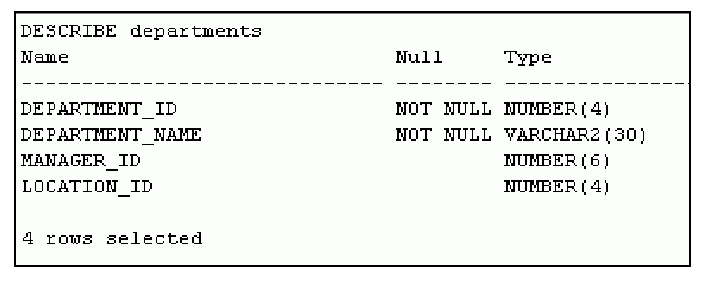
\includegraphics[width=\linewidth]{graphics/4.1.png}
        \end{subfigure}
        \hspace{1em} % Adjusts the space between the images
        \begin{subfigure}[b]{0.45\linewidth}
            \centering
            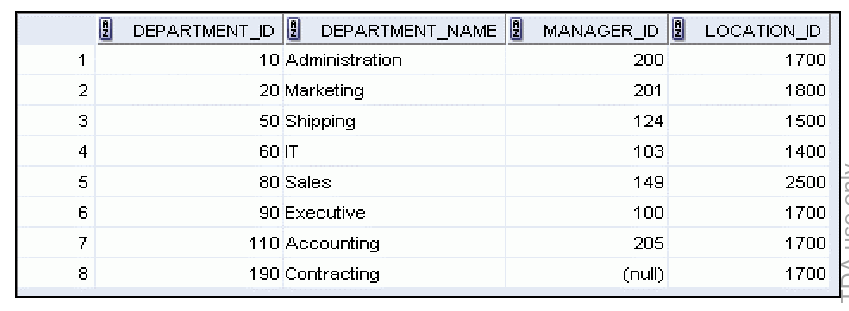
\includegraphics[width=\linewidth]{graphics/4.2.png}
        \end{subfigure}
    \end{figure}
    
    \textbf{Answer: }
    \begin{lstlisting}[language=SQL]
DESCRIBE HR.DEPARTMENTS;
SELECT * FROM HR.DEPARTMENTS;
    \end{lstlisting}
    
    \newpage
    \item You need to determine the structure of the EMPLOYEES table.
    \begin{figure}[h]
        \centering
        \begin{subfigure}[b]{0.3\linewidth}
            \centering
            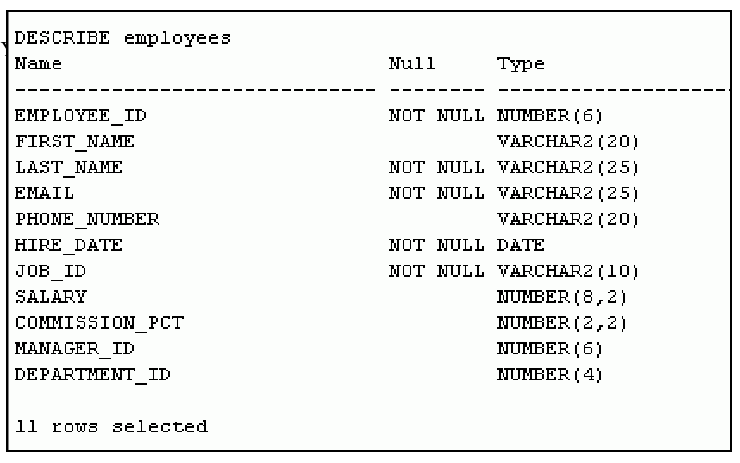
\includegraphics[width=1.5\linewidth]{graphics/5.png}
        \end{subfigure}
    \end{figure}
    
    \textbf{Answer: }
    \begin{lstlisting}[language=SQL]
DESCRIBE HR.EMPLOYEES;
    \end{lstlisting}
    
    \item The HR department wants a query to display the last name, job ID, hire date, and employee ID for each employee, with the employee ID appearing first. Provide an alias \texttt{STARTDATE} for the \texttt{HIRE\_DATE} column. Save your SQL statement to a file named \texttt{lab\_01\_05.sql} so that you can dispatch this file to the HR department.
    Test your query in the \texttt{lab\_01\_05.sql} file to ensure that it runs correctly.
    \begin{figure}[h]
        \centering
        \begin{subfigure}[b]{0.45\linewidth}
            \centering
            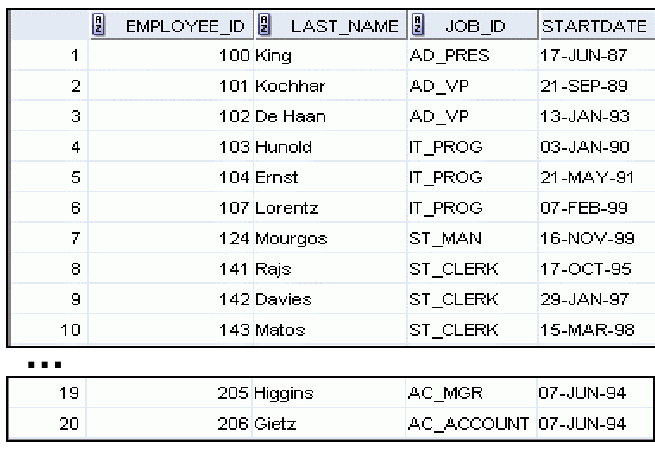
\includegraphics[width=\linewidth]{graphics/6.png}
        \end{subfigure}
    \end{figure}
    
    \textbf{Answer: }
    \begin{lstlisting}[language=SQL]
SELECT EMPLOYEE_ID, LAST_NAME, JOB_ID, HIRE_DATE AS STARTDATE
FROM EMPLOYEES;
    \end{lstlisting}
    
    \newpage
    \item The HR department wants a query to display all unique job IDs from the EMPLOYEES table.
    \begin{figure}[h]
        \centering
        \begin{subfigure}[b]{0.3\linewidth}
            \centering
            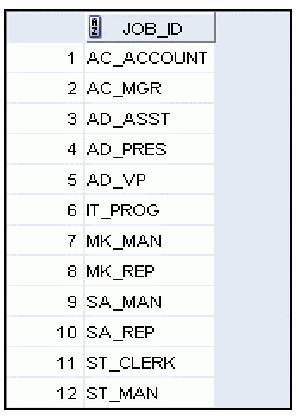
\includegraphics[width=\linewidth]{graphics/7.png}
        \end{subfigure}
    \end{figure}
   
    \textbf{Answer: }
    \begin{lstlisting}[language=SQL]
SELECT DISTINCT JOB_ID
FROM HR.EMPLOYEES;
    \end{lstlisting}
    
\end{enumerate}

\subsection*{Part 3}
\begin{enumerate}[start=8]
    \item The HR department wants more descriptive column headings for its report on employees. Copy
    the statement from \texttt{lab\_01\_05.sql} to a new SQL Worksheet. Name the column headings
    \texttt{Emp \#}, Employee, Job, and Hire Date, respectively. Then run your query again.
    \begin{figure}[h]
        \centering
        \begin{subfigure}[b]{0.5\linewidth}
            \centering
            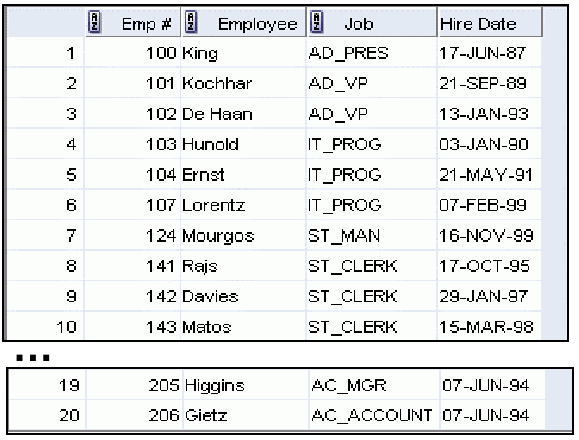
\includegraphics[width=\linewidth]{graphics/8.png}
        \end{subfigure}
    \end{figure}

    \textbf{Answer: }
    \begin{lstlisting}[language=SQL]
SELECT EMPLOYEE_ID AS "Emp #",LAST_NAME AS "Employee", 
JOB_ID AS "Job",HIRE_DATE AS "Hire Date"
FROM EMPLOYEES;
    \end{lstlisting}
    
    \newpage
    \item The HR department has requested a report of all employees and their job IDs. Display the last name concatenated with the job ID (separated by a comma and space) and name the column Employee and Title.
    \begin{figure}[h]
        \centering
        \begin{subfigure}[b]{0.5\linewidth}
            \centering
            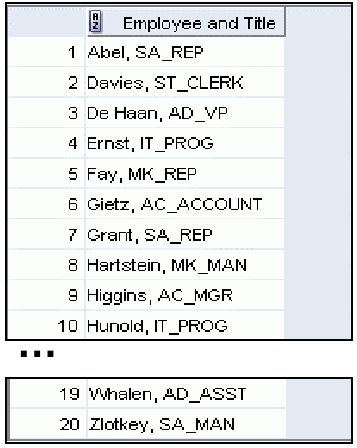
\includegraphics[width=\linewidth]{graphics/9.png}
        \end{subfigure}
    \end{figure}
    
    \textbf{Answer: }
    \begin{lstlisting}[language=SQL, label={lst:concat_query}]
SELECT last_name || ', ' || job_id AS "Employee and Title"
FROM employees;
    \end{lstlisting}
    
    \item To familiarize yourself with the data in the EMPLOYEES table, create a query to display all the data from that table. Separate each column output by a comma. Name the column title THE\_OUTPUT.
    \begin{figure}[h]
        \centering
        \begin{subfigure}[b]{0.4\linewidth}
            \centering
            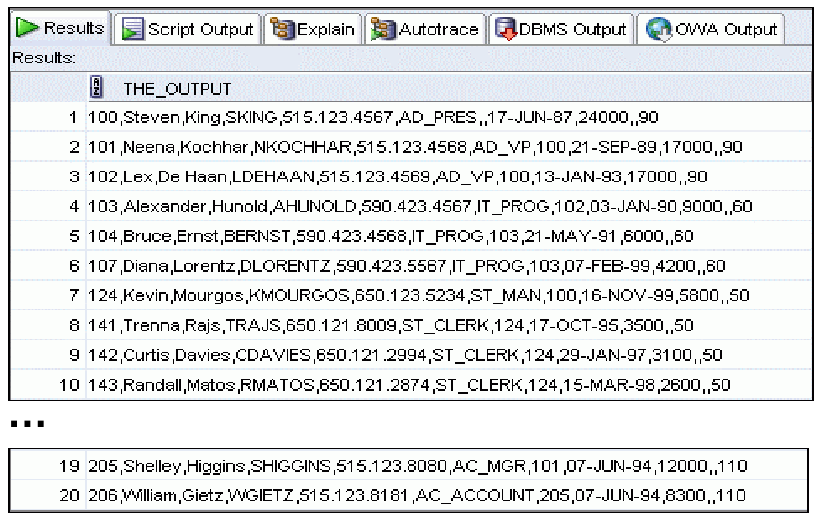
\includegraphics[width=\linewidth]{graphics/10.png}
        \end{subfigure}
    \end{figure}

    \textbf{Answer: }
    \begin{lstlisting}[language=SQL, label={lst:employees_data}]
SELECT Employee_ID||','||First_Name||','||Last_Name||
','||Email||','||Phone_Number||','||Job_ID||','||
Manager_ID||','||Hire_Date||','||Commission_Pct||','||Department_ID AS THE_OUTPUT
FROM HR.EMPLOYEES;
    \end{lstlisting}
    
\end{enumerate}
\newpage
\section*{Chapter 2}
\subsection*{Practice 2}
\begin{enumerate}
    \item Because of budget issues, the HR department needs a report that displays the last name and
salary of employees who earn more than \$12,000. Save your SQL statement as a file named
\texttt{lab\_02\_01.sql}. Run your query.
\begin{figure}[h]
        \centering
        \begin{subfigure}[b]{0.4\linewidth}
            \centering
            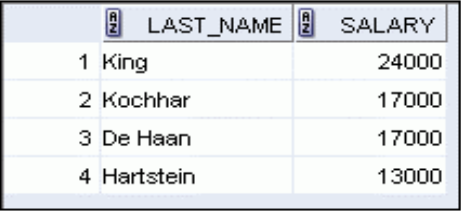
\includegraphics[width=\linewidth]{graphics/21.png}
        \end{subfigure}
    \end{figure}

    \textbf{Answer: }
    \begin{lstlisting}[language=SQL, label={lst:employees_data}]
SELECT Last_Name, Salary
FROM HR.employees
WHERE salary > 12000;
    \end{lstlisting}
        \item Open a new SQL Worksheet. Create a report that displays the last name and department number
for employee number 176. Run the query.
\begin{figure}[h]
        \centering
        \begin{subfigure}[b]{0.4\linewidth}
            \centering
            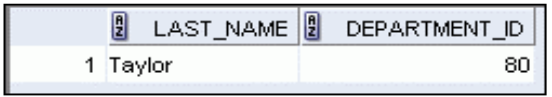
\includegraphics[width=\linewidth]{graphics/22.png}
        \end{subfigure}
    \end{figure}

    \textbf{Answer: }
    \begin{lstlisting}[language=SQL, label={lst:employees_data}]
SELECT last_name, department_id
FROM employees
WHERE employee_id = 176;
    \end{lstlisting}
    \item The HR department needs to find high-salary and low-salary employees. Modify
\texttt{lab\_02\_01.sql} to display the last name and salary for any employee whose salary is not in
the range of \$5,000 to \$12,000. Save your SQL statement as \texttt{lab\_02\_03.sql}.
\begin{figure}[h]
        \centering
        \begin{subfigure}[b]{0.35\linewidth}
            \centering
            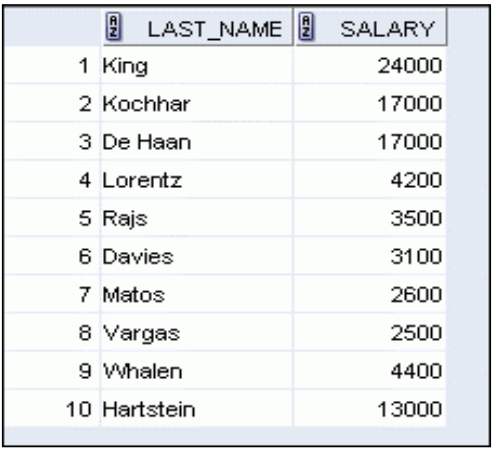
\includegraphics[width=\linewidth]{graphics/23.png}
        \end{subfigure}
    \end{figure}        
    \newpage
    \textbf{Answer: }
    \begin{lstlisting}[language=SQL, label={lst:employees_data}]
SELECT Last_name, Salary
FROM hr.employees
WHERE salary NOT BETWEEN 5000 AND 12000;
    \end{lstlisting}
    \item Create a report to display the last name, job ID, and hire date for employees with the last names
of Matos and Taylor. Order the query in ascending order by the hire date.
\begin{figure}[h]
        \centering
        \begin{subfigure}[b]{0.35\linewidth}
            \centering
            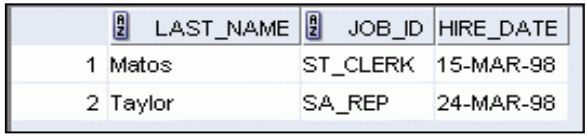
\includegraphics[width=\linewidth]{graphics/24.png}
        \end{subfigure}
    \end{figure}        
    
    \textbf{Answer: }
    \begin{lstlisting}[language=SQL, label={lst:employees_data}]
SELECT 	LAST_NAME, JOB_ID, HIRE_DATE
FROM hr.employees
WHERE last_name IN ('Matos', 'Taylor')
ORDER BY hire_date ASC;
    \end{lstlisting}
    \item Display the last name and department ID of all employees in departments 20 or 50 in ascending
alphabetical order by name.
\begin{figure}[h]
        \centering
        \begin{subfigure}[b]{0.35\linewidth}
            \centering
            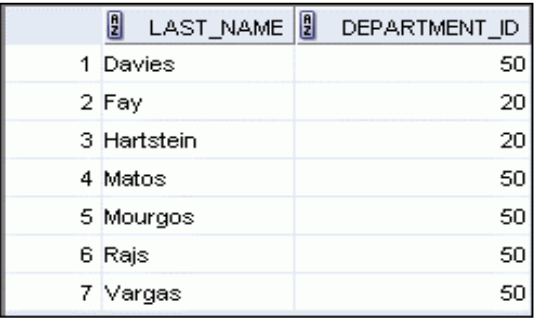
\includegraphics[width=\linewidth]{graphics/25.png}
        \end{subfigure}
    \end{figure}        
    
    \textbf{Answer: }
    \begin{lstlisting}[language=SQL, label={lst:employees_data}]
SELECT last_name, department_id
FROM hr.employees
WHERE department_id IN (20, 50)
ORDER BY last_name ASC;
    \end{lstlisting}
    \item Modify \texttt{lab\_02\_03.sql} to display the last name and salary of employees who earn between
\$5,000 and \$12,000, and are in department 20 or 50. Label the columns Employee and
Monthly Salary, respectively. Resave \texttt{lab\_02\_03.sql} as texttt{lab\_02\_06.sql}. Run the
statement in \texttt{lab\_02\_06.sql}.
\begin{figure}[h]
        \centering
        \begin{subfigure}[b]{0.35\linewidth}
            \centering
            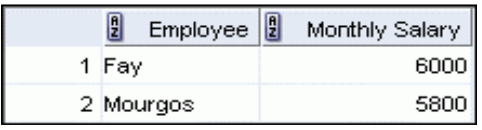
\includegraphics[width=\linewidth]{graphics/26.png}
        \end{subfigure}
    \end{figure}        
    \newpage
    \textbf{Answer: }
    \begin{lstlisting}[language=SQL, label={lst:employees_data}]
SELECT last_name AS Employee, salary AS "Monthly Salary"
FROM hr.employees
WHERE salary BETWEEN 5000 AND 12000
AND department_id IN (20, 50);
    \end{lstlisting}
    \item The HR department needs a report that displays the last name and hire date for all employees
who were hired in 1994.
\begin{figure}[h]
        \centering
        \begin{subfigure}[b]{0.35\linewidth}
            \centering
            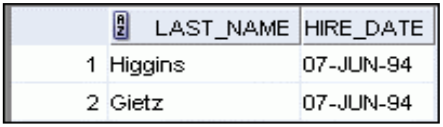
\includegraphics[width=\linewidth]{graphics/27.png}
        \end{subfigure}
    \end{figure}        

    \textbf{Answer: }
    \begin{lstlisting}[language=SQL, label={lst:employees_data}]
SELECT last_name, hire_date
FROM hr.employees
WHERE hire_date LIKE '%94';
    \end{lstlisting}

    \item Create a report to display the last name and job title of all employees who do not have a
manager.
\begin{figure}[h]
        \centering
        \begin{subfigure}[b]{0.35\linewidth}
            \centering
            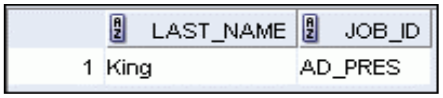
\includegraphics[width=\linewidth]{graphics/28.png}
        \end{subfigure}
    \end{figure}        
    
    \textbf{Answer: }
    \begin{lstlisting}[language=SQL, label={lst:employees_data}]
SELECT LAST_NAME, JOB_ID
FROM hr.employees
WHERE manager_id IS NULL;
    \end{lstlisting}
    \item Create a report to display the last name, salary, and commission of all employees who earn
commissions. Sort data in descending order of salary and commissions.
Use the column numeric position in the ORDER BY clause.
\begin{figure}[h]
        \centering
        \begin{subfigure}[b]{0.6\linewidth}
            \centering
            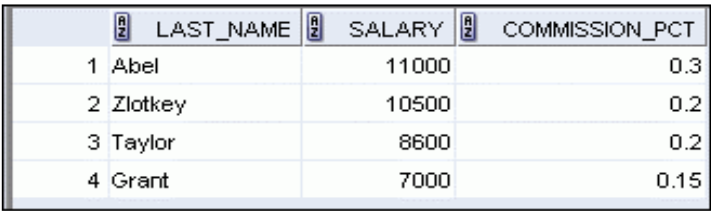
\includegraphics[width=\linewidth]{graphics/29.png}
        \end{subfigure}
    \end{figure}        
    
    \textbf{Answer: }
    \begin{lstlisting}[language=SQL, label={lst:employees_data}]
SELECT last_name, salary, commission_pct
FROM hr.employees
WHERE commission_pct IS NOT NULL
ORDER BY 2 DESC, 3 DESC;
    \end{lstlisting}
    \newpage
    \item Members of the HR department want to have more flexibility with the queries that you are
writing. They would like a report that displays the last name and salary of employees who earn
more than an amount that the user specifies after a prompt. Save this query to a file named
\texttt{lab\_02\_10.sql}. If you enter 12000 when prompted, the report displays the following
results:
\begin{figure}[h]
    \centering
    \includegraphics*[width=0.35\linewidth]{graphics/210.png}
\end{figure}

\textbf{Answer: skipped}
%     \begin{lstlisting}[language=SQL, label={lst:employees_data}]
% SELECT last_name, salary
% FROM employees
% WHERE salary > $user_input;
%     \end{lstlisting}
    \item The HR department wants to run reports based on a manager. Create a query that prompts the
user for a manager ID and generates the employee ID, last name, salary, and department for
that manager's employees. The HR department wants the ability to sort the report on a selected
column. You can test the data with the following values:
\begin{figure}[h]
    \centering
    \includegraphics*[width=.6\linewidth]{graphics/211.png}
\end{figure}

\textbf{Answer: skipped}
    \item Display all employee last names in which the third letter of the name is``a."
\begin{figure}[h]
    \centering
    \includegraphics*[width=.4\linewidth]{graphics/212.png}
\end{figure}

\textbf{Answer: }
    \begin{lstlisting}[language=SQL, label={lst:employees_data}]
SELECT last_name
FROM hr.employees
WHERE last_name LIKE '__a%';
    \end{lstlisting}
    \item Display the last names of all employees who have both an ``a" and an ``e" in their last name.
\begin{figure}[h]
    \centering
    \includegraphics*[width=.4\linewidth]{graphics/213.png}
\end{figure}

\textbf{Answer: }
    \begin{lstlisting}[language=SQL, label={lst:employees_data}]
SELECT last_name
FROM hr.employees
WHERE last_name LIKE '%a%' AND last_name LIKE '%e%';
    \end{lstlisting}
    \item Display the last name, job, and salary for all employees whose jobs are either those of a sales
representative or of a stock clerk, and whose salaries are not equal to \$2,500, \$3,500, or \$7,000.
\begin{figure}[h]
    \centering
    \includegraphics*[width=.4\linewidth]{graphics/214.png}
\end{figure}

\textbf{Answer: }
    \begin{lstlisting}[language=SQL, label={lst:employees_data}]
SELECT last_name, job_id, salary
FROM hr.employees
WHERE job_id IN ('SA_REP', 'ST_CLERK')
AND salary NOT IN (2500, 3500, 7000);
    \end{lstlisting}
    \item Modify \texttt{lab\_02\_06.sql} to display the last name, salary, and commission for all employees
whose commission is 20\%. Resave \texttt{lab\_02\_06.sql} as \texttt{lab\_02\_15.sql}. Rerun the
statement in \texttt{lab\_02\_15.sql}.
\begin{figure}[h]
    \centering
    \includegraphics*[width=.4\linewidth]{graphics/215.png}
\end{figure}

\textbf{Answer: }
    \begin{lstlisting}[language=SQL, label={lst:employees_data}]
SELECT last_name AS Employee, salary AS "Monthly Salary", commission_pct
FROM hr.employees
WHERE commission_pct = 0.20;
    \end{lstlisting}
\end{enumerate}
\end{document}
